\documentclass{article}
\usepackage{amssymb}
\usepackage{amsmath}
\usepackage{mathtools}
\usepackage{cancel}
\usepackage{tikz}
\newtheorem{theorem}{Theorem}
\newtheorem{definition}{Definition}
\newtheorem{corollary}{Corollary}
\newtheorem{proof}{Proof}

\DeclareMathOperator*{\argmin}{argmin}

\begin{document}
\title{EE16B Course Notes}
\author{Anmol Parande}
\date{Spring 2019 - Professors Anant Sahai, Kris Pister, and Jaijeet Roychowdhury}
\maketitle
\section{Discrete Time Models}
Although circuits and other systems function in continuous time, computers can only act in discrete time.
This means the signals they send out to try and control the system are piecewise-continuous, and they can only sense the system at specified intervals $\delta$.
At a discrete time-step $i$, the computer will measure $\vec{x}_d[i]$ and applies the control $\vec{u}[i]$ over the time-interval $[i, i+1]$.
Keep in mind that $t=\delta i$ where $t$ is the continuous time.

\begin{definition}
    The discrete-time state space model is $$\vec{x}_d[i+1]=A_d\vec{x}_d[i]+B_d\vec{u}[i]+\vec{w}[i]$$ where $\vec{w}[i]$ is some disturbance.
\end{definition}

\subsection{Converting between continuous time and discrete time}
To see how to convert between a continuous time model to a discrete time model, consider the following system.
\[
    \begin{array}{c}
        \frac{dx}{dt}=\lambda x+u, u=e^{st}\\
    \end{array}\\
\]

Solving will give $x=\alpha e^{\lambda t}+\beta e^{st}$
Plugging this into the original equation
\[
    \begin{array}{c}
        \alpha \lambda e^{st}+\beta se^{st} = \lambda (\alpha e^{\lambda t}+\beta e^{st})+e^{st}\\
        \text{if}\> \lambda \ne s\\
        \beta s = \beta \lambda + 1 \implies \beta = \frac{1}{s-\lambda}
    \end{array}
    \]
Since the computer only outputs constant signals, $s=0$, so $x=\alpha e^{\lambda t}-\frac{u}{\lambda}$
If $x(0)=x_0$
\[
    \begin{array}{c}
        x(0)=\alpha - \frac{u}{\lambda}=x_0\\
        x = (x_0+\frac{u}{\lambda}e^{\lambda t})-\frac{u}{\lambda}\\
        x = x_0 e^{\lambda t}+u\left(
            \frac{e^{\lambda t}-1}{\lambda}
        \right)
    \end{array}
\]
Notice that at $x(\delta) = x_0 e^{\lambda \delta}+u\left(\frac{e^{\lambda \delta}-1}{\lambda}\right)$
This means that $x[2\delta]$ can be written as $x[2\delta] = x(\delta) e^{\lambda \delta}+u\left(\frac{e^{\lambda \delta}-1}{\lambda}\right)$
because we simply take $x(\delta)$ to be our initial condition.
This allows us to write the discrete time model as
$$x[i+1]=e^{\lambda \delta}x[i]+\left(
    \frac{e^{\lambda \delta}-1}{\lambda}\right) u[i]$$
since the initial condition for the next time-step is simply the value at the previous time-step.
For a vector continuous system, $A_d$ and $B_d$ can be found in the same way by simply solving
the differential equation for each state variable and converting those to discrete time models
and combining the results into matrix-vector form.

\subsection{System Identification}
What would happen if we didn't know what A and B were though? It turns out that we can find it by gathering data about the system and then using least squares.
In the scalar case:
\[
    \begin{array}{c}
        x[i+1]=ax[i]+bu[t]+w[i]\\
        x[1]=ax[0]+bu[0]\\
        x[2]=ax[1]+bu[1]\\
        \vdots\\
        x[m]=ax[m-1]+bu[m-1]
    \end{array}
\]
This means with $m$ observations, we can construct a matrix $D$ and a vector $\vec{s}$ such that we have the least squares problem
\[
    D\vec{p}=\vec{s},\text{ where } \vec{p}=
\left[
    \begin{array}{c}
        a\\
        b\\
    \end{array}
\right]
\]
The same thing can be done in the vector case. We just create multiple parallel systems by multiplying out the rows.
This is called system identification.
\section{Control Theory}
\subsection{Controllability}
\begin{definition}
    A system is controllable if $\forall x^*, \forall x[0], \exists u[0],u[1],...,u[k-1]$ such that $x[k]=x^*$ given that the system starts at $x[0]$
\end{definition}
In words, this means that there exists a sequence of control actions that can eventually get the system anywhere we want it to be from any given initial state.
\begin{theorem}
    If a state is n-dimensional, then a system $$\vec{x}_d[i+1]=A\vec{x}[i]+B\vec{u}[i]+\vec{w}[i]$$ 
    is controllable in k time-steps if $span(B, AB, ..., A^{k-1}B)=\mathbb{R}^n$
\end{theorem}
\begin{proof}
    Without any noise, $\vec{x}_d[i+1]=A\vec{x}[i]+B\vec{u}[i]$
    \[
        \begin{array}{c}
            \vec{x}[1]=A\vec{x}[0]+B\vec{u}[0]\\
            \vec{x}[2]=A\vec{x}[1]+B\vec{u}[1] = A^2\vec{x}[0]+AB\vec{u}[0]+B\vec{u}[i]\\
            \vec{x}[3]=A\vec{x}[2]+B\vec{u}[2] = A^3\vec{x}[0]+A^2B\vec{u}[0]+AB\vec{u}[i]+B\vec{u}[2]\\
            \vdots\\
            \vec{x}[k]=A^k\vec{x}[0]+\sum_{i=0}^{k-1}{A^{k-i-1}B\vec{u}[i]}
        \end{array}
        \]
    Thus the current state is merely a linear combination of vectors in the column spaces of $A^k$ and $B...A^{k-1}$, so if this span is equal to $\mathbb{R}^n$, we can reach every state.
\end{proof}
\begin{definition}
    The controllability matrix is a the matrix whose column space is all the reachable states.
    \[
        \mathcal{C} = \left[
            \begin{array}{c|c|c|c|c}
                A^{k-1}B & A^{k-2}B & ... & AB & B
            \end{array}
        \right]
    \]
\end{definition}
However, if we want to check if a system is controllable in 100 time-steps for a 100 state system, it will be painful to calculate the column space of the controllability matrix.
\\\\It turns out that we can stop checking when $dim(col(B, AB,...,A^{p-1}))=dim(col(B, AB, ..., A^p)), (p \leq k)$ (i.e the dimension of the column space stops growing)
This means we can build the controllability matrix up piece-by-piece and stop early rather than computing the full column space only to fail.
Consider the following proof for why this works.
\begin{proof}
    If $\vec{b}$ is column vector of the matrix B, then $A^p \vec{b}=\sum_{i=0}^{p-1}{\alpha_iA^i\vec{b}}$ since we assume the dimension of the column space has stopped growing,
    so $A^p\vec{b}$ is a linear combination of the vectors preceding it.
    We want to show $\exists \beta_i$ such that $A^{p+1}=\sum_{i=0}^{p-1}{\beta_iA^i\vec{b}}$
    \[
        \begin{array}{c}
            A^{p+1}\vec{b}=A(A^p\vec{b}) =\\\\
            A\sum_{i=0}^{p-1}{\alpha_iA^i\vec{b}} = \sum_{i=0}^{p-1}{\alpha_iA^{i+1}\vec{b}}=\\\\
            \alpha_{p-1}A^p\vec{b}+ \sum_{i=0}^{p-2}{\alpha_iA^{i}\vec{b}}=\\\\
            \alpha_{p-1}\sum_{i=0}^{p-1}{\alpha_iA^i\vec{b}}+\sum_{i=0}^{p-2}{\alpha_iA^{i}\vec{b}}
        \end{array}
        \]
    By writing $A^{p+1}$ as a linear combination of $B, AB,...,A^{p-1}$, we have shown $\beta_i$ exists, so by induction, all future vectors $p+m\leq k$ will be linear combinations of these same vectors, 
    so the dimension will never grow again and we can be justified in stopping early.
\end{proof}
With the controllability matrix, if we want to figure out the controls needed to reach a particular state in $p < k$ steps, all that needs to be done is solve
\[
    \mathcal{C}_p\vec{u} = \vec{x}^* \text{ where } \vec{u} = \left[
            \begin{array}{c}
                \vec{u}[0]\\
                \vec{u}[1]\\
                \vdots\\
                \vec{u}[p]\\
            \end{array}\right], \mathcal{C}_p = \left[
                \begin{array}{c|c|c|c|c}
                    A^{p-1}B & A^{p-2}B & ... & AB & B
                \end{array}
            \right]
\]
\textbf{Important: }this assumes that $\vec{x}[0]=0$. For an arbitrary $\vec{x}[0]$, we would solve $C_p\vec{u}=\vec{x}^*-\vec{x}[0]$.
Look back to where the controllability matrix was derived to see why. 
\subsection{Observability}
Another question we can ask about different systems is whether or not we can figure out exactly where we are.
\begin{definition}
    A system is observable if from a future state $\vec{x}[n]$, the original state $\vec{x}[0]$ is recoverable.
\end{definition}
Often times, we are limited in the measurements we can take, so we might not be able to "see" the entire state vector $\vec{x}[t]$.
Instead, we would only be able to see the output $\vec{y}[t]=C\vec{x}[t]$. To start with, consider what would happen if we applied no inputs to the system.
\[
    \begin{array}{c}
        \vec{y}[0] = C\vec{x}[0]\\\\
        \vec{y}[1] = C\vec{x}[1] = CA\vec{x}[0]\\
        \vdots\\
        \vec{y}[n] = CA^n\vec{x}[0]\\
    \end{array}
\]
\begin{definition}
    \[
    \mathcal{O} = \left[
        \begin{array}{c}
            C\\
            CA\\
            \vdots\\
            CA^i
        \end{array}
    \right],\ \vec{y} = \left[
        \begin{array}{c}
            \vec{y}[0]\\
            \vec{y}[1]\\
            \vdots\\
            \vec{y}[n]\\
        \end{array}
        \right]
\]
is the observability matrix for a system.
\end{definition}
As long as $\mathcal{O}$ is full rank, if we want to recover the state $\vec{x}[0]$, we could apply least squares.
$$\vec{x}[0] = (\mathcal{O}^T\mathcal{O})^{-1}\mathcal{O}^T\vec{y}$$
This brings us the following theorem.
\begin{theorem}
    A system is observable if $\mathcal{O}$ has linearly independent columns.
\end{theorem}
Even if a system has inputs, this kind of analysis still holds.
Define 
$$\vec{x}_f[i]=A\vec{x}[i],\ \vec{y}_f[i]=C\vec{x}_f[0]$$
This is what the system would do without any inputs. If we unroll the recursion in the system, we see
\[
    \begin{array}{c}
        \vec{x}[i] = \vec{x}_f[i]+\sum_{k=0}^{i-1}{A^{i-k-1}B\vec{u}[k]}\\\\
        \vec{y}[i] = \vec{y}_f[i]+\sum_{k=0}^{i-1}{CA^{i-k-1}B\vec{u}[k]}
    \end{array}
\]
Since we know the inputs we applied, and $\vec{x}_f[i]=A^i\vec{x}[i]$, we can easily find $\vec{x}_f[i],\ \vec{y}_f[i]$
and then apply least squares to them to compute the initial state.

\subsection{Stability}
The question of stability is whether or not disturbances will over time control a system if left alone.
Specificically, it is asking if the disturbances are bounded, will the states be bounded too?
\begin{definition}
    Bounded Input, Bounded Output (BIBO) stability means if
    $$|\vec{w}[i]| < \epsilon\text{, then }\exists \delta>0\text{ such that }|\vec{x}[i]| < \delta$$
\end{definition}
To see where this definition comes into play, consider the following scalar systems:
\begin{itemize}
    \item[1.] $x[i+1] = u[i] + w[i]$
    \item[2.] $x[i+1] = \frac{1}{2}x[i] + u[i]+w[i]$ ("Weak" dependence on previous state)
    \item[3.] $x[i+1] = 2 x[i]+u[i]+w[i]$ ("Strong" dependence on previous state)
\end{itemize}
\begin{itemize}
    \item[System 1:] In this system, there is no dependence on the previous state.
    Thus any disturbances are limited to affecting only the next state and no others.
    This makes the system stable because disturbances will not add up.
    To see this mathematically, pretend $u[i] = 0$ since we want to see how the system evolves without doing anything.
    $$|x[i+1]|=|w[i]| < \epsilon, \>\>\> \therefore |x[i]|<\epsilon$$
    Thus we have BIBO stability.
    \item[System 2:] Unlike the previous system, this system has a "weak" dependence on previous states. We consider it "weak" because only half of the previous state influences the next state.
    Intuitively, this system must be BIBO stability then because although disturbances will accumulate, they will be attenuated through an infinite geometric sum. Once again, we will pretend $\vec{u}[i]=0$ to check this mathematically.
    $$|x[i+1]| = \frac{1}{2}x[i]+w[i] < \frac{1}{2}x[i]+ \epsilon$$
    Unrolling the recursive relationship, we see
    $$|x[i+1]| < \epsilon+\frac{1}{2}\epsilon+\frac{1}{4}\epsilon+...+\left( \frac{1}{2} \right)^i\epsilon$$
    $$\lim_{i->\infty}{|x[i+1]|}<\frac{\epsilon}{1-\frac{1}{2}} = 2\epsilon$$
    Thus the system is BIBO stability since $|x[i]| < 2\epsilon$
    \item[System 3:] This system has a "strong" dependence on previous states since the contribution of previous states is doubled each times.
    Intuitively, this means the system must be unstable because small disturbances will be explode over time. To see this mathematically, once again consider what happens if we apply no inputs.
    $$|x[i+1]| = 2x[i]+w[i] < 2x[i]+ \epsilon$$
    Unrolling the recursion,
    $$|x[i+1]| < \epsilon+2\epsilon+4\epsilon+...+2^i\epsilon$$
    $$\lim_{i->\infty}{|x[i+1]|} < \infty$$
    Thus $|x[i]|$ has no bound, so the system is not stable.
\end{itemize}
Note that in the scalar case, as long as $|\lambda| < 1$ for the system $x[i+1]=\lambda x[i]+bu[i]+w[i]$, the system will be stable. Note that this is $\lambda<1$, not $\lambda \leq 1$. That is because when $\lambda=1$, we can see the errors will add up.
\begin{definition}
    A discrete system is marginally stable if $\lambda = 1$
\end{definition}
We call it marginally stable because if there are no disturbances, then it would be stable.
\begin{theorem}
    A vector discrete system $\vec{x}[t+1]=A \vec{x}[t]+B\vec{u}[t]+\vec{w}[t]$ will be stable if the eigenvalues of $A$ are less than 1.
\end{theorem}
\begin{proof}
    If $\exists \> n \> \vec{v}_i$ such that $A\vec{v}_i=\lambda_i\vec{v}_i$, then changing coordinates to the eigenbasis gives
    $$\tilde{A}=
        \left[
        \begin{array}{ccc}
        \lambda_1 &  & 0 \\
         & \ddots &  \\
        0 &  & \lambda_n \\
        \end{array}
        \right] $$
    This means $\vec{\tilde{x}}[t+1]=\tilde{A}\vec{\tilde{x}}[t]+V^{-1}B\vec{u}[t]+V^{-1}\vec{w}[t]$ where $V$ is the matrix whose columns are A's eigenvectors.
    \\\\This is merely n different scalar cases, but we still have to make sure that $|\vec{w}[t]|<\epsilon \implies |V^{-1}\vec{w}[t]|<\kappa$ where $\kappa$ is some bound.
    \\\\Lets say $m=V_{ij}^{-1}$ is the largest entry in $V^{-1}$. In the worst case all $\vec{w}_i[t]$ and all $V_{ij}=m$.
    Then $\forall i, \left[V^{-1}\vec{w}[t]\right]_i \leq n m \epsilon$ where $n$ is the dimension of $V$, which means $|V^{-1}\vec{w}[t]|<\kappa$.
    \\\\Thus we can say that $\tilde{x}[t]$ is BIBO implies that $\vec{x}[t]$ is BIBO.
\end{proof}
It is important to realize that the condition $|\lambda|<1$ holds only for discrete-time systems. If instead our system is continuous (i.e $\frac{d}{dt}\vec{x}(t)=A\vec{x}(t)+B\vec{u}(t)$),
then the system will only be stable if $Re\{\lambda\}<0$. To see why, consider the following simple linear system with initial condition $x_0$.
\[
    \begin{array}{c}
        \frac{d}{dt}x(t) = \lambda x(t)\\
        \therefore x(t) = x_0 e^{\lambda t}
    \end{array}
\]
Clearly if $\lambda > 0$, this system will grow infinitely large. The same analysis applies to vector cases.
\begin{theorem}
    \begin{itemize}
        \item[]
        \item[1. ] A continuous system is stable if the real part of its eigenvalues are less than 0 (i.e $Re\{\lambda\} < 0$)
        \item[2. ] A discrete system is stable if $|\lambda| < 1$
    \end{itemize}
\end{theorem}

\subsubsection{Stability for a general A matrix}
Notice that checking stability based on the eigenvalues requires the matrix $A$ to be diagonalizable becase we need to check all of its eigenvalues.
This leaves open the question of what happens when $A$ is not diagonalizable, meaning there are not n distinct eigenvalues.
In order to resolve this problem, we are going to need a new matrix form called Schur Upper Triangular Form.
\begin{definition}
    The Schur Upper Triangular form of a matrix A is
    \[
        \left[
            \begin{array}{cccc}
                \lambda_1 & * & * & ... \\
                0 & \lambda_2 & * & ... \\
                0 & 0 & \ddots & \\
                \vdots & \vdots &  & 
            \end{array}
        \right]
        \]
    It is an upper triangular matrix with eigenvalues on the diagonal. The eigenvalues may equal = 0.
\end{definition}
Schur form allows us to easily find the characteristic polynomial of the matrix and solve the problem of stability.
To see why it helps with stability, consider the following proof.
\begin{proof}
    $$\tilde{x}[t+1]=\tilde{A}\tilde{x}[t]+\tilde{w}[t]$$
    If $\tilde{A}$ is in Schur form, then the nth component is
    $$\tilde{x}_n[t+1]=\lambda_n\tilde{x}_n[t]+\tilde{w}_n[t]$$
    so if $|\lambda_n| < 1$, then $\tilde{x}_n$ is BIBO stable.
    Likewise, for the n-1th component
    $$\tilde{x}_{n-1}[t+1]=\lambda_{n-1}\tilde{x}_{n-1}[t]+s\tilde{x}_n[t]+\tilde{w}_{n-1}[t]$$
    $s$ is one of the $*$ entries in the upper part of Schur form. It doesn't matter what it is because $\tilde{x}_n[t]$ is BIBO, so $s\tilde{x}_n[t]$ is also BIBO.
    \\\\As a result $\tilde{x}_{n-1}[t]$ will be BIBO if $|\lambda_{n-1}|<1$ and $|\lambda_n| < 1$.
    Since the component $\tilde{x}_{n-i}[t+1]$ depends on $\tilde{x}_n[t], \tilde{x}_{n-1}[t],...$, as long as $\tilde{x}_n[t], \tilde{x}_{n-1}[t],...$ are stable, $\tilde{x}_{n-i}[t+1]$ will be stable too.
    \\\\Thus as long as all $|\lambda_i|<1$, then Schur form tells us whether or not the system is stable.
\end{proof}
Now that we know how it works, we need to know how to find a basis $U$ such that $\tilde{A}=U^{-1}AU$. As a bonus, it would be helpful if $U$ is orthonormal.
To make things easier later, we'll define $M_n = A$. Since all matrices have at least one eigenpair, we can choose
$$M\vec{v}_1=\lambda_1\vec{v}_1, ||\vec{v}_1||=1$$

Using Gram-Schmidt, we can now pick $n-1$ vectors $\vec{r}_i$ such that
$$U_1 = \vec{v}_1, \vec{r}_1, ..., \vec{r}_{n-1}$$ is an orthonormal basis. Note, the vectors $\vec{r}_i$ form a $n \times (n-1)$ matrix $R_{n-1}$
Lets look at $M_n$ in the $U_1$ basis.
\[
    U_1^{-1}M_nU_1=
    \left[
        \begin{array}{c}
            \vec{v}_1^T \\\\
            R_{n-1}^T
        \end{array}
    \right]
    M_n
    \left[
        \begin{array}{cc}
            \vec{v}_1 & R_{n-1}
        \end{array}
    \right] = 
    \left[
        \begin{array}{cc}
            \vec{v}_1^T M_n \vec{v}_1 & \vec{v}_1^T M_n R_{n-1} \\\\
            R_{n-1}^T M_n \vec{v}_1^T & R_{n-1}^T M_n R_{n-1}
        \end{array}
    \right] = 
    \left[
        \begin{array}{c|c}
            \lambda_1 & * \\
            \hline\\
            0 & R_{n-1}^T M R_{n-1}
        \end{array}
    \right]
\]
We can see that we are getting closer to where we want to be, so lets continue with the matrix $M_{n-1}$.
We can find a vector of size $n-1$ such that
$$M_{n-1}\vec{v_2}=\lambda_2\vec{v}_2, ||\vec{v}_2||=1$$
Extending this to an orthonormal basis $U_2$, we get a matrix $R_{n-2}$
\[
    \left[
        \begin{array}{c}
            \vec{v}_2^T \\\\
            R_{n-2}^T
        \end{array}
    \right]
    M_{n-1}
    \left[
        \begin{array}{cc}
            \vec{v}_2 & R_{n-2}
        \end{array}
    \right] = 
    \left[
        \begin{array}{cc}
            \vec{v}_2^T M_{n-1} \vec{v}_2 & \vec{v}_2^T M_{n-1} R_{n-2} \\\\
            R_{n-1}^T M_{n-1} \vec{v}_1^T & R_{n-1}^T M_{n-1} R_{n-1}
        \end{array}
    \right] = 
    \left[
        \begin{array}{c|c}
            \lambda_2 & * \\
            \hline\\
            0 & R_{n-2}^T M_{n-1} R_{n-2}
        \end{array}
    \right]
\]
We can keep repeating this by saying $M_{n-2} = R_{n-2}^T M_{n-1} R_{n-2}$, but we need to know if our $\lambda_2$ has any relation to the eigenvalues of A.
Lets say $$U_2 = \vec{v}_1, \vec{x}, rest$$ is a basis where $\vec{x}$ has some dependence on $\vec{v}_2$.
There aren't many options for what $\vec{x}$ and the rest of the basis vectors could be, so let's try.
$$\vec{x}=R_{n-1}\vec{v}_2,\ rest = R_{n-1}R_{n-2}$$ because this will get us the appropriate sized vectors.
Notice this basis will also be orthonormal because $\vec{v}_1^T R_{n-1}=0$ and $\vec{v_2}R_{n-1}^TR_{n-1}R_{n-2}=\vec{v_2}^TR_{n-2}=0$
Lets see how $M_n$ looks in the basis $U_2$ to see if we are getting closer to Schur form.
\[
    \begin{array}{c}
        U_2^-1M_nU_2 = 
        \left[
            \begin{array}{c}
                \vec{v}_1^T \\\\
                (R_{n-1}\vec{v}_2)^T\\\\
                (R_{n-1}R_{n-2})^T
            \end{array}
        \right]
        M_n
        \left[
            \begin{array}{ccc}
                \vec{v}_1^T & R_{n-1}\vec{v}_2 & R_{n-1}R_{n-2}
            \end{array}
        \right] = \\\\
        \left[
            \begin{array}{ccc}
                \vec{v}_1^T M_n \vec{v}_1 & \vec{v}_1^T M_n R_{n-1}\vec{v}_2 & \vec{v}_1^T M_n R_{n-1}R_{n-2}\\\\
                (R_{n-1}\vec{v}_2)^T M_n \vec{v}_1^T & (R_{n-1}\vec{v}_2)^T M_n R_{n-1}\vec{v}_2 & (R_{n-1}\vec{v}_2)^T M_n R_{n-1}R_{n-2}\\\\
                (R_{n-1}R_{n-2})^T M_n \vec{v}_1 & (R_{n-1}R_{n-2})^T M_n R_{n-1}\vec{v}_2 & (R_{n-1}R_{n-2})^T M_n R_{n-1}R_{n-2}
            \end{array}
        \right] = \\\\
        \left[
            \begin{array}{c|c|c}
                \lambda_1 & *  & *\\
                \hline & &\\
                0 & \lambda_2 & *\\
                \hline & &\\
                0 & 0 & (R_{n-1}R_{n-2})^T M_n R_{n-1}R_{n-2}\\
                \vdots & \vdots
            \end{array}
        \right]
    \end{array}
\]

The $\lambda_2$ showed up because
$$\vec{v}_2^TR_{n-1}^TM_nR_{n-1}\vec{v}_2)=\vec{v}_2M_{n-1}\vec{v}_2=\lambda_2$$
This tells us we can continue with this process to get to Schur form.
To get to Schur Form, all we need to do is
\begin{itemize}
    \item[] Let $M_n=A$
    \item[Loop:]
    \item[] Find $\lambda_i, \vec{v}_i$ such that $M_{n+1-i}\vec{v}_i=\lambda_i\vec{v}_i,\ ||\vec{v}_i||=1$
    \item[] Find $R_{n-i}$ such that $R_{n-i}^T\vec{v}_i=0$ and $R_{n-i}^TR_{n-i}=I_{n-1}$
    \item[] $M_{n-i} = R_{n-i}^TM_{n+1-i}R_{n-i}$
    \item[End Loop]
    \item[] $U = \vec{v_1},\ R_{n-1}\vec{v}_2,\ R_{n-1}R_{n-2}\vec{v}_2,\ ...,\ (\prod_{j=1}^{k}{R_{n-j}})\vec{v}_{k+1}$
\end{itemize}
Thus $\tilde{A}=U^TAU$ will give the Schur Form of the matrix A.
Notice that $(U^TAU)^T=U^TA^TU$. This forms the basis for \textbf{Spectral Theorem}.
\begin{theorem}[Spectral Theorem]
    Every real symmetric matrix has real eigenvalues can be orthogonally diagonalized
\end{theorem}
Two consequences of spectral theorem are that if the symmetric matrix $A$ is real, then
\begin{itemize}
    \item[1. ] All eigenvalues are real
    \item[2. ] All eigenvectors are real
\end{itemize}

\subsection{Closed Loop Control}
Lets say we have a system which is modeled by $\vec{x}[t+1]=A \vec{x}[t]+B\vec{u}[t]+\vec{w}[t]$
We must choose our inputs $\vec{u}[t]$ based on only $\vec{x}[t]$ since we can't observe the disturbances. How should we choose our inputs to control the system?
If we try $\vec{u}[t]=k\vec{x}[t]$, then
\[
    \begin{array}{c}
        \vec{x}[t+1]=A\vec{x}[t]+Bk\vec{x}[t]+\vec{w}[t]\\
        \vec{x}[t+1]=(A+Bk)\vec{x}[t]+\vec{w}[t]
    \end{array}
\]
Which means that if we choose $K$ appropriately, we can potentially change the behavior of the system.
Consider the following simple scalar case example
\[
    \begin{array}{c}
        x[t+1]=3x[t]+u[t]+w[t]\\
        u[t] = kx[t]\\
        x[t+1] = (3+k)x[t]+w[t]
    \end{array}
\]
Notice that even if the system is initially unstable, we can set our $k$ to make it stable since the domain of $\lambda=3+k$ is $\infty$
\\\\What if we have a system $\vec{x}[t+1]=A\vec{x}[t]+\vec{b}u[t]+\vec{w}[t]$ where $A, \vec{b}$ are controllable, but we only get a scalar input $u[t]$.
Can we find a set of feedback gains $\vec{f}^T=[f_0, f_1, ..., f_{k-1}]$ such that $u[t]=-\vec{f}^T\vec{x}[t]$ makes $A-\vec{b}\vec{f}^T$ have the eigenvalues we want?
\break \break
We know how to easily solve scalar cases like $z[t+1]=az[t]+u[t]$, but it is hard to get this from a vector case because we only have a simple input, so we will be limited in how we can set our eigenvalues this way.
Since this won't work, consider the folowing recursive system.
$$z[t+1]=a_{k-1}z[t]+a_{k-2}z[t-1]+...+a_0z[t-(k-1)]+u[t]$$
This is definetly controllable since our input $u[t]$ could potentially be any value in $\mathbb{R}$.
Moreover, if we choose $u[t]=-\sum_{i=0}^{k-1}{f_i z[t-(k-1)+i]}$, we can create any recurrence relation we want.
\\\\For example, if we wanted $z[t+1]=d_{k-1}z[t]+d_{k-2}z[t-1]+...+d_0z[t-(k-1)]$, then $f_i=a_i-d_i$
Writing this in vector form, we get
\[
    \begin{array}{c}
    \vec{z}[t+1]=A_z z[t]+\vec{b}u[t] \\
    \\
    \vec{z}[t] = \left[
        \begin{array}{c}
            z[t-(k-1)]\\
            \vdots\\
            z[t-2]\\
            z[t-1]\\
            z[t]
        \end{array}
    \right]
    \end{array}
\]
Notice that the vector $\vec{z}[t]$ here is different from the scalar $z[t]$ which it is made up of. Each "state" here is a scalar quantity, but to represent the recursive relationship properly, we collect all of the previous states in a vector to define the next state.
\break\break
Given our definition of $\vec{z}[t]$ (which are the scalar values of previous states), we can fill in values for $A_z$ and $\vec{b}$
\[
    A_z = \left[
        \begin{array}{cccccc}
            0 & 1 & 0 & 0 & ... & 0\\
            0 & 0 & 1 & 0 & ... & 0\\
            0 & 0 & 0 & 1 & ... & 0\\
            \vdots & & & & \ddots & \vdots\\
            a_0 & a_1 & a_2 & ... & & a_{k-1}
        \end{array}
    \right],\>
    \vec{b} = \left[
        \begin{array}{c}
            0\\
            0\\
            0\\
            \vdots\\
            1
        \end{array}
    \right]
\]
To understand where these come from, thing of the $A_z$ matrix "scrolling down" the state vector $\vec{z}[t]$ to get how it influences $\vec{z}[t+1]$.
All the rows except the last are 0's and 1's since the previous states can't change, but the last row determines the next state.
\\\\Notice that all entries in the b-vector are 0 except the last since we can't affect the past with present control.
We can assume $a_0\ne 0$ since we defined the recurrence to have length $k$. Breaking $A_z$ into its block components gives us some more insight to its structure.
\[
    A_z = \left[
        \begin{array}{c}
            \begin{array}{c|c}
                0 & I_{k-1}\\
            \end{array} \\
            \hline \\
            \vec{a}^T
        \end{array}
    \right]
\]
We can check through multiplication that this system will be controllable.
\begin{definition}
    A system is in Controllable Canonical Form if
    \[
    A_z = \left[
        \begin{array}{c}
            \begin{array}{c|c}
                0 & I_{k-1}\\
            \end{array} \\
            \hline \\
            \vec{a}^T
        \end{array}
    \right],\ \vec{b}_z = \left[
        \begin{array}{c}
            0\\
            0\\
            0\\
            \vdots\\
            1
        \end{array}
    \right]
\]
\end{definition}
Let's try finding the eigenvalues of $A_z$. If $A_z$ is large, it'll be hard to calculate the characteristic polynomial, so instead lets guess their form and figure them out that way.
\[
    \vec{v}_\lambda = \left[
        \begin{array}{c}
            1\\
            *\\
            *\\
            \vdots
        \end{array}
    \right]
    \]
Where * is any element.
We know $A_z\vec{v}_\lambda=\lambda v_\lambda$, and since $A_z$ scrolls the vector down, we can see that the second * must be $\lambda$. Applying this same logic to the second *, it must be $\lambda^2$.
Continuing this, we get
\[
    \vec{v}_\lambda = \left[
        \begin{array}{c}
            1\\
            \lambda\\
            \lambda^2\\
            \vdots\\
            \lambda^{k-1}
        \end{array}
    \right]
    \]
If we wanted to find the characteristic polynomial, we could look at the last entry in $A_z\vec{v}_\lambda$
\[
    \begin{array}{c}
        \sum_{i=0}^{k-1}{a_i\lambda_i}=\lambda*\lambda^{k-1}=\lambda_k\\\\
        \text{Rearranging: }\lambda_k-\sum_{i=0}^{k-1}{a_i\lambda_i} = 0
    \end{array}
\]
Notice this is the characteristic polynomial of $A$. That means if we want to simply find what the CCF form of the system looks like, rather than computing the transformation $\mathbb{H}\mathbb{G}^{-1}$,
we can instead use the fact that $a_0, a_1, ... a_{k-1}$ are the coefficients of the characteristic polynomial.
\\\\Along the same train of thought, if we want to design feedback controls
\\$\vec{u}[t]=-\vec{f}^T\vec{z}[t]$ to make the system stable,
all we need to do is set $f_i = a_i - d_i$ where $d_i$ are the desired coefficients of the desired characteristic polynomial.
To see why, refer back to the scalar case or try multiplying out $(A_z-\vec{b}_z\vec{f}^T)$.
 Thus CCF is useful because it makes it extremely easy to place the eigenvalues for any system.
\\\\Now that we know about this matrix form, the question becomes: can we transform any controllable system with matrix A into controllable canonical form?
(i.e can we make $\vec{x}[t+1]=A\vec{x}[t]+\vec{b}u[t]$ into $\vec{z}[t+1]=A_z\vec{z}[t]+\vec{b}_zu[t]$)
\\\\We know that $\vec{b}, A\vec{b}, A^2\vec{b}, ... A^{k-1}\vec{b}$ are linearly independent since our system is controllable. Let this define basis $\mathbb{G}$. If we write the matrix A in the basis of G, we get $\tilde{A}=G^{-1}AG$.
The naming choice is very appropriate here because this matrix multiplication will be painful by hand, so lets look for another way to get $\tilde{A}$.
\\\\Remember that any linear transformation is defined by what it does to the basis vectors. We know
\[
    \tilde{b} = G^{-1}\vec{b} = \left[
        \begin{array}{c}
            1\\
            0\\
            0\\
            \vdots\\
        \end{array}
    \right]
\]
since $\vec{b}$ is the first basis vector of $\mathbb{G}$. Thus,
\[
    \tilde{A}\tilde{\vec{b}}=G^{-1}A\vec{b} = \left[
        \begin{array}{c}
            0\\
            1\\
            0\\
            \vdots\\
        \end{array}
    \right],\>
    \tilde{A}^2\tilde{\vec{b}} = G^{-1}A^2\vec{b} = \left[
        \begin{array}{c}
            0\\
            0\\
            1\\
            \vdots\\
        \end{array}
    \right] ...
\]
This gives us $k$ columns of $\tilde{A}$. For the last column must be a linear combination of all the basis vectors, so $\tilde{A}^k\tilde{\vec{b}}=\sum_{i=0}^{k-1}{\alpha_i\tilde{A}^i\tilde{\vec{b}}}$
This means
\[
    \tilde{A} = \left[
        \begin{array}{cccc}
            0 & 0 & ... & \alpha_0\\
            1 & 0 & ... & \alpha_1\\
            0 & 1 & ... & \alpha_2\\
            \vdots & & \ddots & \vdots\\
            0 & ... & 1 & \alpha_{k-1}
        \end{array}
    \right]
    \]
which is $A_z^T$.
This means that our basis $\mathbb{G}$ is essentially the controllability matrix $\mathcal{C}$ except with the rows reordered.
\\\\Now we have a basis $\mathbb{G}$ with $(\tilde{A}, \tilde{b}$), but we want a basis $\mathbb{H}$ with $(\tilde{A}^T, \vec{b}_z)$
We want $\tilde{A}^T, \vec{b}_z$ to be controllable, which means $\vec{b}_z, \tilde{A}^T\vec{b}_z,...,(\tilde{A}^T)^{k-1}\vec{b}_z$ are linearly independent.
Let's construct a matrix H which will take us from a coordinates in basis $\mathbb{H}$ to coordinates in the basis $\mathbb{G}$. 
\[
    \mathbb{H} = \left[
        \begin{array}{c|c|c|c}
            \vec{b}_z & \tilde{A}^T\vec{b}_z & ... &(\tilde{A}^T)^{k-1}\vec{b}_z
        \end{array}
    \right]
\]
Once we have the matrix H, to get $(\tilde{A}^T, \vec{b}_z)$ from $(A, \vec{b})$,
we can apply the change of coordinates $G^{-1}H$ so $\vec{x}_z[t]=HG^{-1}\vec{x}[t]$ and put our entire system into controllable canonical form.
\subsection{Linearization}
Up until now, we have been assuming our systems are linear. To understand what this means, we must first understand what linearity means.
First, let's define what we know as a function.
\begin{definition}
    A function is a simple mapping from a domain to a range (i.e y(t)=L(u(t))). 
    To evaluate y(t), we only need to know u(t), making the function "memory-less"
\end{definition}
\begin{definition}
    A function $f(x)$ is linear iff
    \begin{itemize}
        \item $\forall \alpha, \forall x \in \mathbb{R}, f(\alpha x) = \alpha f(x)$ (Scaling)
        \item $\forall u, \forall v \in \mathbb{R}, f(u + v) = f(u)+f(v)$ (Superposition)
    \end{itemize}
\end{definition}
Notice that by this definition, any linear function must necessarily have $f(0)=0$ since otherwise with $\alpha = 1, x=0, f(1*0)=f(0)=1*f(0)\ne 0$
\\\\These conditions can be simplified down into a single expression 
$$f(\alpha u + v) = \alpha f(u) + f(v), \forall u, \forall v, \forall \alpha \in \mathbb{R}$$
If we can find a single setting of $(u, v, \alpha)$ for which this equation does not hold, then our function is not linear.
\\\\If we have a scalar nonlinear function we can linearize it in a simple way. Remember that the Taylor series expansion of a function around a certain point is
$$ f(x) = \frac{f(c)}{0!}+\frac{f'(c)}{1!}(x-c)+\frac{f''(c)}{2!}(x-c)^2+... = \sum_{i=0}^{\infty}{\frac{f^{(i)}}{i!}(x-c)^i}$$
where $c$ is some expansion point we choose. Lets say we choose some point $x^*$ and decide to linearize around that point.
The tangent line to the function is
$$f_L(x)=f'(x^*)(x-x^*)+f(x^*)$$
However, $f(0)\ne 0$, so this tangent line is still not linear. To linearize it, we can change coordinates.
\[
    \begin{array}{c}
        m = \frac{df}{dx}|_x\\\\
        f(x^*+\delta x)= f(x^*)+m \delta x\\\\
        \delta y = f(x^*+\delta x) - f(x^*)\\\\
        f(x^*+\delta x) = f(x^*)+\delta y = f(x^*)+m \delta x\\\\
        \delta y = m \delta x
    \end{array}
\]

Thus the linearized expression is in terms of the "error" $\delta y$, a.k.a how far it deviates from what it was at the point of linearization.
While this makes sense for functions, how does it apply to systems. Systems are more than simple functions, they are functionals.
\begin{definition}
    A functional y(t) = L\{u(t)\} is a function which requires knowing the entire u in order to evaluate it.
\end{definition}
A good example of a functional is
$$ L\{u(t)\}=\int_{\tau - 1}^{\tau}{u(t)d\tau}$$

The definition of linearity for functionals is virtually the same as for a normal function.
\begin{definition}
    A system $L\{\}$ is linear iff
    \begin{itemize}
        \item $\forall \alpha\in \mathbb{R}, \forall u(t), L\{\alpha u(t)\} = \alpha L\{u(t)\}$ (Scaling)
        \item $\forall u(t), \forall v(t), L\{u(t) + v(t)\} = L\{u(t)\}+L\{v(t)\}$ (Superposition)
    \end{itemize}
\end{definition}
With this definition, we can now formally define how to linearize a non-linear system.
Take the system $\frac{d}{dt}x(t) = f(x(t))+bu(t)$ where $f$ is a nonlinear function and $b$ is a scalar multiplier.
To linearize the system:
\begin{itemize}
    \item[1.] Choose a constant with time input $u(t) = u^*$
    \item[2.] Find a solution $x(t)=x^*$ to the system
            $$\frac{dx^*}{dt}=f(x^*)+bu^* \implies f(x^*)=-bu^*$$
    \item[3.] Linearize $f(x)$ around $x^*$
            $$f(x) \approx f(x^*)+\frac{df}{dx}|_{x^*} (x-x^*)$$
    \item[4.] Use the linearization of $f$ to make the differential equation linear
            \[
                \begin{array}{c}
                    \frac{dx}{dt} = f(x^*)+\frac{df}{dx}|_{x^*} (x(t)-x^*)+bu(t)\\\\
                    \text{Let }\delta x = x(t)-x^*, \delta u = u(t) - u^*\\\\
                    \frac{d}{dt}(\delta x +x^*) = f(x^*)+\frac{df}{dx}|_{x^*} \delta x + b (u^*+\delta u)\\\\
                    \frac{d}{dt}\delta x = \cancelto{0}{f(x^*)+bu^*} + \frac{df}{dx}|_{x^*} \delta x + b \delta u(t)\\\\
                    \frac{d}{dt}\delta x =  \frac{df}{dx}|_{x^*} \delta x + b \delta u(t)
                \end{array}
            \] 
\end{itemize}
Note that this only works assuming that $\delta x$ is small, so when linearizing our systems, 
we must check that this property is true otherwise our linearization may be invalid. 
\\\\To see why, consider the system $\frac{d}{dt}=-sin(x)$. Try linearizing about $x^*=0$.
\[
    \begin{array} {c}
        \frac{d}{dt}\delta x = -\delta x\\\\
        \therefore \delta x = \delta x(0)e^{-t}
    \end{array}
\]
Since $\delta x$ is the "error" of our approximation, we can see that
$$\lim_{\delta x \to \infty}{\delta x} = 0$$
This means the linearization is stable, and our approximation is legimitate.
However, if we linearize about $x^*=\pi$
\[
    \begin{array} {c}
        \frac{d}{dt}\delta x = \delta x\\\\
        \therefore \delta x = \delta x(0)e^{t}\\\\
        \lim_{\delta x \to \infty}{\delta x} = \infty
    \end{array}
\]
Thus this linearization is unstable and will diverge over a long period of time, so it is not a good linearization.
\\\\These concepts of linearization extend beyond simple 1D functions. For example, the linearization of a 2D function is
$$f(x^*+\delta x, u^*+\delta u) \approx f(x^*, u^*)+\frac{\partial f}{\partial x}|_{x^*, u^*}\delta x+\frac{\partial f}{\partial u}|_{x^*, u^*}\delta u$$
We can further generalize the idea of linearization to vector functions.
\[
    f(\vec{x})=\left[
        \begin{array}{c}
            f_1(x_1, x_2)\\
            f_2(x_1, x_2)
        \end{array}
        \right] \text{ where } \vec{x} = \left[
            \begin{array}{c}
                x_1\\
                x_2
            \end{array}
            \right]
    \]

If we linearize each of the functions inside the vector, we get
\[
    \begin{array}{c}
        f(\vec{x^*}+\delta\vec{x^*})=\left[
            \begin{array}{c}
                f_1(x_1^*+\delta x_1, x_2^*+\delta x_2)\\
                f_2(x_1^*+\delta x_1, x_2^*+\delta x_2)
            \end{array}
        \right] \\\\
        f_1(x_1^*+\delta x_1, x_2^*+\delta x_2) \approx f_1(x_1^*, x_2^*)+\frac{\partial f_1}{\partial x_1}|_{x_1^*, x_2^*}\delta x_1+\frac{\partial f_1}{\partial x_2}|_{x_1^*, x_2^*}\delta x_2\\\\
        f_2(x_1^*+\delta x_1, x_2^*+\delta x_2) \approx f_2(x_1^*, x_2^*)+\frac{\partial f_2}{\partial x_1}|_{x_1^*, x_2^*}\delta x_1+\frac{\partial f_1}{\partial x_2}|_{x_1^*, x_2^*}\delta x_2\\\\
        \therefore f(\vec{x^*}+\delta\vec{x^*})=\left[
            \begin{array}{c}
                f_1(x_1^*+\delta x_1, x_2^*+\delta x_2)\\
                f_2(x_1^*+\delta x_1, x_2^*+\delta x_2)
            \end{array}
        \right] = \left[
            \begin{array}{c}
                f_1(x_1^*, x_2^*)\\
                f_2(x_1^*, x_2^*)
            \end{array}
            \right] + \left[
                \begin{array}{cc}
                    \frac{\partial f_1}{\partial x_1} & \frac{\partial f_1}{\partial x_2} \\\\
                    \frac{\partial f_2}{\partial x_1} & \frac{\partial f_1}{\partial x_2}
                \end{array}
                \right] |_{x_1^*, x_2^*} \left[
                    \begin{array}{c}
                        \delta x_1\\
                        \delta x_2
                    \end{array}
                    \right]
    \end{array}
\]

The matrix with partial derivatives is known as the \textbf{Jacobian} and is denoted either $\nabla f$ or $J$
Thus a succinct form the linearization of a vector system is
$$ f(\vec{x^*}+\delta\vec{x})=f(\vec{x^*})+J_x f (\delta \vec{x})$$
For multiargument functions,
$$ f(\vec{x^*}+\delta\vec{x}, \vec{u^*}+\delta \vec{u})=f(\vec{x^*}, \vec{u^*})+J_x \delta \vec{x}+J_u \delta \vec{u}$$
\subsection{Planning}
With all of these tools, we can now tackle the problem of planning. With closed loop control, we know we can keep a system near a specific state even if the system is unstable by itself due to disturbances.
We can use this fact to keep our system close to a specified "open loop" trajectory by redefining our equilibrium position is along a specific trajectory.
\subsubsection{Open Loop Control}
Lets say we have a controllable system $\frac{d}{dt} \vec{x}[t]=A\vec{x}[t]+\vec{b}u[t] + \vec{w}[t]$, a desired trajectory $\vec{x}_n[t]$, and a set of inputs that will take us along that trajectory $u_n[t]$.
We can define $\vec{v}[t] = \vec{x}[t]-\vec{x}_n[t]$ and $u_v[t] = u[t] - u_n[t]$ as the trajectory deviation and input deviation respectively.
Writing this equation in terms of the deviations gives us
\[
    \begin{array}{c}
        \frac{d}{dt}\vec{x}[t]=A\vec{x}[t]+\vec{b}u[t]+ \vec{w}[t]\\\\
        \frac{d}{dt}(\vec{v}[t]+\vec{x}_n[t]) = A(\vec{v}[t] + \vec{x}_n[t]) + \vec{b}(u_v[t] + u_n[t])+ \vec{w}[t]\\\\
        \frac{d}{dt}\vec{v}[t] + \cancelto{}{\frac{d}{dt}\vec{x}_n[t])} = (A\vec{v}[t] + \vec{b}u_v[t]) + \cancelto{}{(A\vec{x}_n[t] + u_n[t])} + \vec{w}[t]\\\\
        \frac{d}{dt}\vec{v}[t] = A\vec{v}[t]+\vec{b}u_v[t] + \vec{w}[t]
    \end{array}
\]
Since our original system was controllable, this system must be controllable as well. In fact, it will have all the same characteristics as the original system (controllability, stability, observability) since they share the same $A$ and $\vec{b}$.
\\\\This tells us that if the original system was not stable, then we will not be able to follow the trajectory $\vec{x}[n]$ since our deviation from the trajectory $\vec{v}[t]$ can blow up from disturbances.
Lets apply feedback control to make sure the deviation does not grow expnentially large.
\[
    u_v[t] = 
    \left[
        \begin{array}{cccc}
            f_0 & f_1 & f_2 ...
        \end{array}
    \right] \vec{v}[t]
\]
This will let us control the deviation from the desired trajectory.
This lets us compute the controls we need to follow the trajectory by inserting this result back into the formula for $u[t]$
\[
    \begin{array}{c}
        u[t] = u_n[t]+u_v[t] = u_n[t]+\left[
            \begin{array}{cccc}
                f_0 & f_1 & f_2 & ...
            \end{array}
        \right] \vec{v}[t] \\\\
        u[t] = u_n[t]+\left[
            \begin{array}{cccc}
                f_0 & f_1 & f_2 & ...
            \end{array}
        \right] (\vec{x}[t]-\vec{x}_n[t])
    \end{array}
\]

\subsubsection{Minimum Energy Control}
For any generic system, we know that if the system is controllable, we can use controls to take it to any state we want.
For example, if the state is 10-dimensional, then it will take a maximum of 10 time-steps to move anywhere.
But what should we do if we want to get to a system in 100 time-steps instead?
\\\\One approach is to move to the desired state $x^*$ in 10 time-steps and then do nothing for the remaining 90 time-steps,
 but this is a bad solution because the dynamics of the environment may prevent our system from staying in one place at a time (imagine a jumping robot that needs to reach a height at a specific time. Continuously jumping up and down waste's a lot of energy)
\\\\Another idea is to visit random states for 90 time-steps and spend the next 10 moving towards the goal, but once again, this wastes energy.
Ideally, we should take a "natural" path which uses the dynamics of the environment as much as possible.
\\\\A good example of this is a satellite such as Voyager. It could continuously use fuel to get where it needs to go, but it is much more energy efficient for it to use the gravity of planets to gain speed instead.
This concept is known as minimum energy control.
\begin{definition}
    The minimum energy control problem is to find $\argmin{||\vec{u}||}$ such that $C\vec{u}=\vec{x}^*$ where 
    C is the controllability matrix for the system, $\vec{x}^*$ is a desired state, and $\vec{u}$ is a vector of inputs applied at each time-step (assuming our inputs are scalar).
\end{definition}
Like most problems, this one is difficult to solve in its original state. Since the controllability matrix is of dimension $n \times k$ with $k > n$ ($n$ is the dimension of the state and $k$ is how many time-steps we want to reach our goal in), 
the matrix must have a null space. Moving around inside this null space is a waste of energy because it doesn't get us close to $x^*$. This tells us two things about how we might solve this problem.
\begin{itemize}
    \item[1. ] We should change coordinates to an orthonormal basis because it might make the problem easier to solve without changing the length of the vectors.
    \item[2. ] We should try an isolate the null space when we construct a basis because we don't want to move in those directions.  
\end{itemize}
Mathematically, this means we want
\[
    V = \left[
        \begin{array}{cccc}
            \vec{v_1} & \vec{v_2} & ... & \vec{v_k}
        \end{array}
    \right] \text{ such that } V^TV=I \text{ and } C\vec{v_i} = 0\text{ for } i > n
\]
In the new basis, the problem becomes
\[
    \argmin{||\tilde{\vec{u}}||} \text{ such that } CV\tilde{\vec{u}}=\vec{x}^*
\]
Notice that the product $CV\tilde{\vec{u}}$ is a linear combination of only the first $n$ basis vectors.
\[
    C \left[
        \begin{array}{cccc}
            | & | & & |\\
            \vec{v_1} & \vec{v_2} & ... & \vec{v_k}\\
            | & | & & |
        \end{array}
    \right] \left[
        \begin{array}{c}
            \tilde{u}_1\\
            \vdots\\
            \tilde{u}_n
        \end{array}
    \right] = C (\tilde{u}_1\vec{v}_1+...+\tilde{u}_n\vec{v}_n)
\]
This is because $C\vec{v}_i\tilde{u}_i=0$ for $i>n$ based on the properties we want out of V.
Clearly it would be very useful to have this basis $V$ because then we could let $\tilde{u}_i=0$ for $i > n$ to minimize $||\tilde{\vec{u}}||$.
\\\\At this point, we should try constructing V. We know that any symmetric matrix can be orthogonally diagonalized because of spectral theorem.
Lets try finding a symmetric matrix $Q$ such that $Null(Q)=Null(C)$ because then the eigenvectors of Q which form a basis for $Null(Q)$ will also form an orthogonal basis for $Null(C)$. Notice that $C^TC$ has this property.
\begin{proof}
    $\vec{v}\in Null(C) \implies C\vec{v}=\vec{0}$, then $C^TC\vec{v} \implies \vec{v} \in Null(C^TC)$
    $\vec{v} \in Null(C^TC) \implies C^TC\vec{v}=\vec{0}$, $C\vec{v} \cdot C\vec{v}=\vec{v}^TC^TC\vec{v}=\vec{0}\implies \vec{v}\in Null(C)$
    Since any vector in $Null(C)$ belongs to $Null(C^TC)$ and vice versa, the two null spaces are the same.
\end{proof}
Let's say $V$ is the orthonormal basis of eigenvectors of Q which we know exists from the spectral theorem.
If we order our eigenvectors such that their corresponding eigenvalues are related by $\lambda_1 \ge \lambda_2 \ge ... \ge \lambda_k \ge 0$,
then we get
\[
    \begin{array}{c}
        \Lambda = V^T(C^TC)V=\left[
        \begin{array}{cccc}
            \lambda_1 & 0 & ... & 0\\
            0 & \lambda _2 & & \vdots\\
            \vdots & & \ddots & \\
            0 & ... & & \lambda_k
        \end{array}
    \right]\\
    \text{ where only the first } n \text{ diagonal entries are not zero}
    \end{array}
\]
An interesting fact about these eigenvalues is that $\lambda_i = ||C\vec{v}_i||^2$
\begin{proof}
    \[
        \begin{array}{c}
            C^TC\vec{v}_i = \lambda_i \vec{v}_i\\
            \vec{v}_i^TC^TC\vec{v}_i = ||C\vec{v}_i||^2 \\
            \vec{v}_i^TC^TC\vec{v}_i = \vec{v}_i^TQ\vec{v}_i = \lambda \vec{v}_i^T\vec{v}_i = \lambda_i\\
            \therefore \lambda_i = ||C\vec{v}_i||^2
        \end{array}
    \]
\end{proof}
For convenience (and for reasons which will be clear later), lets defined $\sigma_i=\sqrt{\lambda_i} = ||C\vec{v}_i||$ to remove the exponent.
A curious fact about the eigenvectors is that the matrix C does not change their orthogonality.
\begin{proof}
    $(C\vec{v}_i^T)(C\vec{v}_j)=\vec{v}_i^TC^TC\vec{v_j}=\vec{v}_i^T\lambda_j \vec{v}_j = 0$
\end{proof}
This means the vectors $C\vec{v}_i$ for $i \le n$ form an orthonormal basis for $\mathbb{R}^n$ (we disregard $C\vec{v}_i)$ for $i > n$ since these are merely zero vectors).
Lets normalize this basis so $$\vec{w}_i=\frac{C\vec{v}_i}{||C\vec{v}_i||}=\frac{C\vec{v}}{\sigma_i}$$
Now that we have extracted everything useful out of our basis $V$, let's return to the original problem of $\argmin{\tilde{\vec{u}}}$.
\[
    \begin{array}{c}
        CV\tilde{\vec{u}}=\sum_{i=1}^{n}{C\vec{v}_i\tilde{u}_i} =\\\\
        \sum_{i=1}^{n}{\sigma_i\tilde{u}_i\vec{w}_i} = \vec{x}^*
    \end{array}
\]
By inspection, we can see that if we let $\tilde{u}_i=\frac{\vec{w}^T_ix^*_i}{\sigma_i}$, then the sum will work out.
This means the following $\tilde{\vec{u}}$ will solve our problem.
\[
    \tilde{\vec{u}} = \left[
        \begin{array}{c}
            \frac{\vec{w}^T_1x^*_1}{\sigma_1}\\
            \vdots\\
            \frac{\vec{w}^T_nx^*_n}{\sigma_n}\\
            0\\
            \vdots\\
            0
        \end{array}
    \right]
\]
And from these we can find the actual controls by $\vec{u}_{opt}=V\tilde{\vec{u}}$.
\section{SVD and PCA}
The analysis which we did above reveals an incredibly interesting fact.
\[
    \begin{array}{c}
        \tilde{u}_i=\vec{v}_i^T\vec{u}\\
        C\vec{u}=\sum_{i=1}^{n}{C\vec{v_i}\tilde{u}_i}=\\\\
        \sum_{i=1}^{n}{(\sigma_i\vec{w_i}\vec{v}^T_iu_i)}=\\\\
        \sum_{i=1}^{n}{(\sigma_i\vec{w_i}\vec{v}^T_i)} \vec{u}\\\\
        \therefore C = \sum_{i=1}^{n}{(\sigma_i\vec{w_i}\vec{v}^T_i)} = W\Sigma V^T
    \end{array}
\]
This shows that the matrix $C\in \mathbb{R}^{m \times n}$ can be factored into a product of three matrices.
$W\in \mathbb{R}^{m \times m}$ has orthonormal columns, $\Sigma \in \mathbb{R}^{m \times n}$ has $\sigma_i$ on the diagonal, and $V^T \in \mathbb{R}^{n \times n}$ also has orthonormal columns.
Together, these matrices form the \textbf{Singular Value Decomposition} of $C$. The values $\sigma_i$ on the diagonal are called the \textbf{singular values}. Note that C was a generic matrix, which means \textbf{any} matrix can be factored in this way. 
\begin{definition}
    Any matrix $A\in \mathbb{R}^{m\times n}$ can be factored such that $A = U\Sigma V^T$
     where $U\in \mathbb{R}^{m\times m}$, $\Sigma \in \mathbb{R}^{m \times n}$, $V\in \mathbb{R}^{n \times n}$
     with $U,V$ having orthonormal columns and $\Sigma$ is diagonal. 
\end{definition}

\subsection{Computing the SVD}
The procedure for computing the SVD of a matrix procedes exactly what was done above to find minimum energy control.
First, we find the eigenpairs of $A^TA$ and these become our $V$ matrix and $\lambda_i=\sigma_i^2$. To find U, we let $\vec{u}_i=\frac{A\vec{v}_i}{\sigma_i}$ for all $\sigma \ne 0$ and then use Gram Schmidt to find the rest of the basis.
However, if the matrix $A$ is $m \times n$, if $A^TA$ will be $n \times n$. If $n > m$, then this means we have to compute more eigenvectors. Instead, it would be less work to find the eigenvectors of $AA^T$ and make those the vectors in U.
In general, the SVD can be found as follows.
\begin{itemize}
    \item[] If $m > n$
    \item[1. ] $\vec{v}_i$ are the eigenvectors of $A^TA$, $\sigma_i=\sqrt{\lambda_i}$
    \item[2. ] $\vec{u_i}=\frac{A\vec{v_i}}{\sigma_i} \forall \sigma_i \ne 0$
    \item[3. ] Extend the basis of vectors ${\vec{u}_1, \vec{u}_2, ..., \vec{u_n}}$ into an orthonormal basis for $\mathbb{R}^m$ using Gram Schmidt.
    \item[] If $m < n$
    \item[1. ] $\vec{u}_i$ are the eigenvectors of $AA^T$, $\sigma_i=\sqrt{\lambda_i}$
    \item[2. ] $\vec{v}_i=\frac{A^T\vec{u}_i}{\sigma_i} \forall \sigma_i \ne 0$
    \item[3. ] Extend the basis of vectors ${\vec{v}_1, \vec{v}_2, ..., \vec{v_m}}$ into an orthonormal basis for $\mathbb{R}^n$ using Gram Schmidt.
\end{itemize}
Extending a basis can be a lot of work, so there also exists the compact form of the SVD.
\begin{definition}
    Any matrix $A\in \mathbb{R}^{m\times n}$ can be factored such that $A = U\Sigma V^T$
     where $U\in \mathbb{R}^{m\times k}$, $\Sigma \in \mathbb{R}^{k \times k}$, $V\in \mathbb{R}^{k \times n}$
     with $U,V$ having orthonormal columns and $\Sigma$ is square. $k$ is the number of nonzero singular values.
     This is known as the compact form of the SVD.
\end{definition}
The compact form is found by following the same procedure of finding the SVD but not extending any bases.
\subsection{Outer Product Form of SVD}
In the SVD of a matrix A, $A = \sum_{i=1}^{n}{(\sigma_i\vec{w_i}\vec{v}^T_i)}$, the term $\vec{w}\vec{v}^T$ is a special type of product known as an \textbf{outer product}.
If $\vec{w}\in \mathbb{R}^n$ and $\vec{v}\in \mathbb{R}^m$, then $\vec{w}\vec{v}^T$ produces a $n \times m$ matrix of rank 1.
All matrix multiplications can be expressed as a sum of outer products.
\[
    \left[
        \begin{array}{cccc}
            | & | & & |\\
            \vec{x}_1 & \vec{x}_2 & ... & \vec{x}_m\\
            | & | & & |
        \end{array}
    \right]\left[
        \begin{array}{ccc}
            - & \vec{y}_1^T & -\\
            - & \vec{y}_2^T & -\\
             & \vdots & \\
             - & \vec{y}_m & -
        \end{array}
    \right] = \sum_{i=1}^{m}{\vec{x}_i\vec{y}_i^T}
\]
This is why $A = \sum_{i=1}^{n}{(\sigma_i\vec{w_i}\vec{v}^T_i)}$ is known as the \textbf{outer product form} of the SVD.
The outer product form shows us that every matrix can be expressed as a sum of outer products a.k.a a sum of rank 1 matrices.
The outer products which correspond to higher singular values have more "weight" in making up the original matrix. 

\subsection{Approximating a matrix}
Another outcome of outer products is that theoretically, if we have a large matrix (such as an image),
we can retain most of its information but remember fewer numbers by throwing away the outer products which correspond to lower singular values.
i.e for a matrix $A$ which is $p \times q$
$$A = \sum_{i=1}^{m}{\sigma_i\vec{u}_i\vec{v}_i^T} \approx \sum_{i=1}^{k}{\sigma_i\vec{u}_i\vec{v}_i^T}$$
Where $m$ is the smaller dimension of the matrix and $k < m$. The error of this approximation can also be found easily.
$$A - \hat{A} = \sum_{i=k+1}^{m}{\sigma_i\vec{u}_i\vec{v}_i^T}$$
These are merely the thrown away terms. We can reduce this to a number by taking the Frobenius Norm of the error matrix.
\begin{definition}
    The Froebenius norm of a matrix $A$, written $||A||_F$, is the square root of the sum of the squares of each element.
    $$||A||_F^2 = \sum_{i=1}^{n}{\sum_{j=1}^{m}{|a_{ij}|^2}}$$
\end{definition}
With this definition, it is easy to see that the error of our approximation depends only on the approximations.
$$||A-\hat{A}||_F^2 = \sum_{i=k+1}^{m}{\sigma_i^2}$$
The following theorem contains useful features of the Frobenius Norm and can be proved fairly easily.
\begin{theorem}
    \begin{itemize}
        \item[]
        \item[1. ] $||A||_F^2=Tr\{A^TA\}$
        \item[2. ] For an orthonormal matrix $U$, $||A||_F=||UA|_F=||AU||_F$
    \end{itemize}
\end{theorem}
\subsubsection{The Moore-Penrose Pseudoinverse}
SVD gives us insight into how we might find a solution to $A\vec{x}=\vec{y}$ when $A\in \mathbb{R}^{m\times n}$
where $n > m$. If $Rank(A)=m$, then there will be infinitely many solutions. We can easily construct one solution by "undoing" the SVD.
\[
    \begin{array}{c}
        A\vec{x}=\vec{y}\\
        U\Sigma V^T\vec{x} = \vec{y}\\
        \Sigma V^T \vec{x} = U^T\vec{y}\\
        V^T\vec{x} = \left[
            \begin{array}{cccc}
                \frac{1}{\sigma_1} & 0 & ... & 0\\
                0 & \frac{1}{\sigma_2} & ... & 0\\
                0 & 0 & \ddots & \\
                \vdots & \vdots & \vdots & \vdots\\
                0 & 0 & 0 & 0\\
                \vdots & \vdots & \vdots & \vdots
            \end{array}
            \right]U^T \vec{y}\\
        \vec{x} = V \left[
            \begin{array}{cccc}
                \frac{1}{\sigma_1} & 0 & ... & 0\\
                0 & \frac{1}{\sigma_2} & ... & 0\\
                0 & 0 & \ddots & \\
                \vdots & \vdots & \vdots & \vdots\\
                0 & 0 & 0 & 0\\
                \vdots & \vdots & \vdots & \vdots
            \end{array}
            \right]U^T \vec{y}
    \end{array}
\]
This "undoing" is known as the Moore-Penrose Pseudoinverse.
\begin{definition}
    The Moore-Penrose Psuedoinverse is $A^\dagger = V\tilde{\Sigma}U^T$ where
    \[
        \tilde{\Sigma} = \left[
            \begin{array}{cccc}
                \frac{1}{\sigma_1} & 0 & ... & 0\\
                0 & \frac{1}{\sigma_2} & ... & 0\\
                0 & 0 & \ddots & \\
                \vdots & \vdots & \vdots & \vdots\\
                0 & 0 & 0 & 0\\
                \vdots & \vdots & \vdots & \vdots
            \end{array}
            \right]
    \]
\end{definition}
$\tilde{\Sigma}$ can be thought of as $(\Sigma^T)^{-1}$ where divisions by 0 are ignored.
\\\\Notice that the Moore-Penrose Psuedo-inverse gives us the exact solution to the minimum energy control problem which we saw earlier.
\subsection{PCA}
PCA is a technique which is closely related to the SVD. It applies to matrices which represent data.
Lets say we have a matrix $A \in \mathbb{R}^{n \times m}$ in which each row represents a data vector.
To make analysis more accurate, it is nice to have all of our data centered around zero.
To do this, find the mean of each column $\mu_1, ..., \mu_m$ and subtract out the column average from each data point.
\[
    \tilde{A} = \left[
        \begin{array}{cccc}
            x_{11} - \mu_1 & x_{12} - \mu_2 & ... &x_{1m} - \mu_m\\
            x_{21} - \mu_1 & x_{22} - \mu_2 & ... &x_{2m} - \mu_m\\
             & & \vdots & \\
             x_{n1} - \mu_1 & x_{n2} - \mu_2 & ... &x_{nm} - \mu_m\\
        \end{array}
    \right]
\]
\begin{definition}
    $$ S \triangleq \frac{1}{n}\tilde{A}^T\tilde{A}$$
    is the covariance matrix of $A$. $n$ is the number of datapoints,
    and $\tilde{A}$ is the mean-centered A matrix.
    \[
        S = \left[
            \begin{array}{ccc}
                s_{11} & ... & s_{1m}\\
                \vdots & \ddots & \vdots\\
                s_{m1} & ... & s_{mm}
            \end{array}
        \right]
    \]
\end{definition}
\begin{theorem}
    The covariance matrix S has the following properties.
    \begin{itemize}
        \item $S^T = S$ (i.e it is symmetric)
        \item $S_{ii} \ge 0, S_{ii} \in \mathbb{R}$
        \item $|s_{ij}| \le |s_{ii}s_{jj}|$
    \end{itemize}
\end{theorem}
Notice that the diagonals contain the statistical variance of each "feature" of the data (each feature corresponds to a different column).
(Remember that the variance $\sigma_x^2 = \frac{1}{n}\sum_{i=1}^{n}{x_i-\mu}$ for data points $x_1, ..., x_n$).
To simplify notation, lets rename each diagonal entry to be $s_i^2=s_{ii}$.
With the covariance matrix, we can now find the correlation matrix, another statistical matrix which tells us the linear correlation between data.
\begin{definition}
    \[
        R \triangleq \left[
            \begin{array}{cccc}
                1 & \frac{s_{12}}{s_1s_2} & ... & \frac{s_{1m}}{s_1s_m}\\
                \frac{s_{21}}{s_2s_1} & \ddots & &\\
                \vdots & & \ddots & \vdots\\
                \frac{s_{m1}}{s_ms_1} & ... & ... & 1
            \end{array}
        \right]
    \]
\end{definition}
The R matrix contains the correlations between each feature. All of the terms on its diagonal are 1, and $R^T=R$.
Each $-1 \le r_{ij} \le 1$. A correlation of 1 means complete positive linear correlation while correlation of -1 means complete negative linear correlation.
A correlation of 0 means no correlation at all. The correlation matrix is nice to do analysis on because it tells us how each feature is correlated.
However, it is painful to calculate and if any of the diagonal entries of the covariance matrix is 0, then the R matrix will be undefined.
PCA is a way to get around these issues.
\\\\PCA finds principal components of the data.
\begin{definition}
    The principal components of a matrix $A$ are the eigenvectors of the covariance matrix $S$
    i.e, since $S$ is symmetric, it can be othorgonally diagonalized into $S = P\Lambda P^T$.
    The principal components are merely the vectors in P.
\end{definition}
Principal components are the "axes" along which the data varies the most.
Principal component analysis involves projecting the mean centered data $\tilde{A}$ onto the principle components ($\hat{A}=\tilde{A}P)$).
Note that $\hat{A}$ will also be mean centered since
\[
    \begin{array}{c}
        \frac{\left[
        \begin{array}{ccccc}
            1 & 1 & 1 & 1 & ...
        \end{array}
    \right]}{n} \tilde{A}P = 0 \\\\
    \therefore \frac{\left[
        \begin{array}{ccccc}
            1 & 1 & 1 & 1 & ...
        \end{array}
    \right]}{n} \hat{A} = \frac{\left[
        \begin{array}{ccccc}
            1 & 1 & 1 & 1 & ...
        \end{array}
    \right]}{n} \tilde{A}P = 0
    \end{array}
\]
The reason why the eigenvectors of $S$ are the axes along which the data varies the most is because 
if we compute $\hat{S}$, the covariance of the projected data, we get a diagonal matrix.
$$\hat{S}=\frac{1}{n}\hat{A}^T\hat{A} = \frac{1}{n}P^T\tilde{A}^T\tilde{A}P=P^TSP=\Lambda$$
The fact that covariance matrix is 0 means thats all of the variances between different features are 0,
effectively meaning that we have "decoupled" the features.
This gives us a good basis to analyze our data for tasks like classification because features are not interacting with each other.
Notice that the matrix $P$ is the same as the matrix $V$ in the SVD of $\tilde{A}$ since 
$$S=\frac{1}{n}\tilde{A}^T\tilde{A} = \frac{1}{n}V\Sigma^TU^TU\Sigma V^T = \frac{1}{n}V\Sigma^T\Sigma V^T$$
Thus $\Lambda = \frac{\Sigma^T \Sigma}{n}$. This gives us an easy way to do PCA since we can just do SVD.
\section{Signal Processing}
\subsection{Interpolation}
\begin{definition}
    Interpolation is the process of reconstructing a signal from a series of samples.
\end{definition}
For example, if we have an audio signal and record the waveform's value at specific intervals,
then interpolation allows us to approximate what the orginal waveform looked like using only the samples.
\subsubsection{Interpolation with basis functions}
One way which we can do interpolation is with basis functions.
\begin{definition}
    A basis function $\phi(t)$ is a function where
    \[
        \phi(t) = \left\{
            \begin{array}{c}
                1, \text{ if } t = 0\\
                0,\text{ if } t=k\Delta,\ k \ne 0
            \end{array}
        \right\}
     \]
     where $\Delta$ is the time interval at which samples were taken.
\end{definition}
If we have samples $y_1, y_2,..., y_n$, then the reconstructed function $f(x)$ is
$$f(x) = \sum_{i=1}^{n}{y_i\phi(t-\Delta)}$$
By interpolating with basis functions, our resulting point hits every sample properly
(which is accomplished by shifting $\phi$ by $\Delta$ for each datapoint).
\begin{definition}
    Zero-Order-Hold interpolation is when
    \[
        \begin{array}{c}
            \phi(t) = \left\{
            \begin{array}{c}
                1, \text{ if } t = 0\\
                0, \text{ else}
            \end{array}
        \right\}\\\\
        \begin{tikzpicture}
            \draw[thick,<->] (-1.5, 0) -- (1.5,0);
            \draw[thick,->] (0,0) -- (0,2);
            \foreach \x in {-1,0,1}
                \draw (\x cm,1pt) -- (\x cm,-1pt) node[anchor=north] {$\x$};
            \foreach \y in {1}
                \draw (1pt,\y cm) -- (-1pt,\y cm) node[anchor=east] {$\y$};
                \draw[scale=1,domain=0:1,smooth,variable=\x,blue] plot ({\x},{1});
        \end{tikzpicture}
        \end{array}
    \]
\end{definition}
When used in interpolation, Zero-Order-Hold looks like the following.
\[
    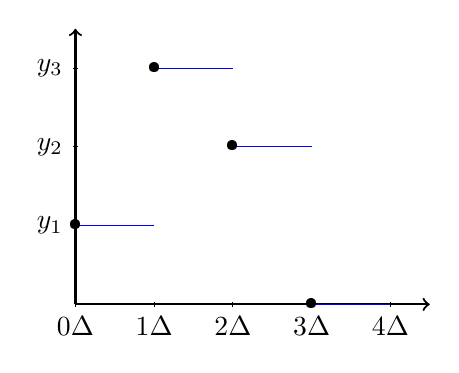
\begin{tikzpicture}
        \draw[thick,->] (0, 0) -- (4.5,0);
        \draw[thick,->] (0,0) -- (0,3.5);
        \foreach \x in {0,1, 2, 3, 4}
            \draw (\x cm,1pt) -- (\x cm,-1pt) node[anchor=north] {$\x \Delta$};
        \foreach \y in {1,2,3}
            \draw (1pt,\y cm) -- (-1pt,\y cm) node[anchor=east] {$y_{\y}$};
        \draw[scale=1,domain=0:1,smooth,variable=\x,blue] plot ({\x},{1});
        \draw[scale=1,domain=2:3,smooth,variable=\x,blue] plot ({\x},{2});
        \draw[scale=1,domain=1:2,smooth,variable=\x,blue] plot ({\x},{3});
        \draw[scale=1,domain=3:4,smooth,variable=\x,blue] plot ({\x},{0});
        \foreach \Point in {(0,1), (2,2), (1,3), (3, 0)}{
            \node at \Point {\textbullet};
        }
    \end{tikzpicture}
\]
Notice that Zero-Order hold interpolation is not continuous, nor is it differentiable.
In a sense, it is the simplest form of interpolation. Another really simply interpolation is piecewise-linear interpolation.
\begin{definition}
    The Piecewise linear basis function is
    \[
        \phi(t) = \left\{
        \begin{array}{c}
            x + 1, \text{ if } -\Delta < x <= 0\\
            -x + 1, \text{ if } 0 <= x < \Delta\\
            0, \text{ else}
        \end{array}
        \right\}
    \]
    \[
        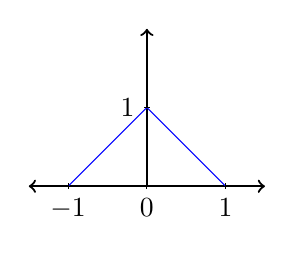
\begin{tikzpicture}
            \draw[thick,<->] (-1.5, 0) -- (1.5,0);
            \draw[thick,->] (0,0) -- (0,2);
            \draw[blue] (-1, 0) -- (0, 1);
            \draw[blue] (0, 1) -- (1, 0);
            \foreach \x in {-1,0,1}
                \draw (\x cm,1pt) -- (\x cm,-1pt) node[anchor=north] {$\x$};
            \foreach \y in {1}
                \draw (1pt,\y cm) -- (-1pt,\y cm) node[anchor=east] {$\y$};
        \end{tikzpicture}
    \]
\end{definition}
Piece-wise linear interpolation is equivalent to connecting each sample.
\[
    \begin{array}{cc}
        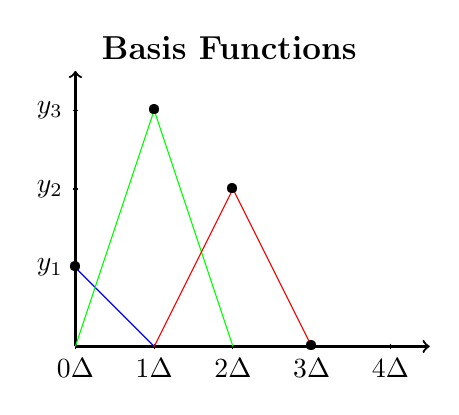
\begin{tikzpicture}
            \draw[thick,->] (0, 0) -- (4.5,0);
            \draw[thick,->] (0,0) -- (0,3.5);
            \foreach \x in {0,1, 2, 3, 4}
                \draw (\x cm,1pt) -- (\x cm,-1pt) node[anchor=north] {$\x \Delta$};
            \foreach \y in {1,2,3}
                \draw (1pt,\y cm) -- (-1pt,\y cm) node[anchor=east] {$y_{\y}$};
                \draw[blue] (0, 1) -- (1, 0);
                \draw[green] (0, 0) -- (1, 3);
                \draw[green] (1, 3) -- (2, 0);
                \draw[red] (1, 0) -- (2, 2);
                \draw[red] (2, 2) -- (3, 0);
            \foreach \Point in {(0,1), (2,2), (1,3), (3, 0)}{
                \node at \Point {\textbullet};
            }
            \node[above,font=\large\bfseries] at (current bounding box.north) {Basis Functions};
        \end{tikzpicture}
        &
        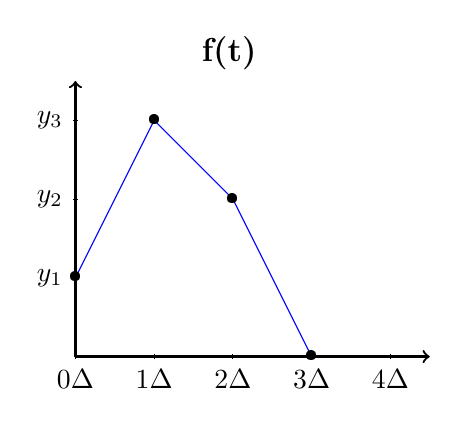
\begin{tikzpicture}
            \draw[thick,->] (0, 0) -- (4.5,0);
            \draw[thick,->] (0,0) -- (0,3.5);
            \foreach \x in {0,1, 2, 3, 4}
                \draw (\x cm,1pt) -- (\x cm,-1pt) node[anchor=north] {$\x \Delta$};
            \foreach \y in {1,2,3}
                \draw (1pt,\y cm) -- (-1pt,\y cm) node[anchor=east] {$y_{\y}$};
            \draw[blue] (0, 1) -- (1, 3);
            \draw[blue] (1, 3) -- (2, 2);
            \draw[blue] (2, 2) -- (3, 0);
            \foreach \Point in {(0,1), (2,2), (1,3), (3, 0)}{
                \node at \Point {\textbullet};
            }
            \node[above,font=\large\bfseries] at (current bounding box.north) {f(t)};
        \end{tikzpicture}
    \end{array}
\]
Piece-wise linear interpolation gives us a function which is continuous but not differentiable.
\begin{definition}
    Sinc interpolation has the basis function
    \[
        \phi(t) = \left\{
            \begin{array}{c}
                1, \text{ if } t = 0\\\\
                \frac{sin(\pi t)}{\pi t}, t \ne 0
            \end{array}
            \right\}
    \]
    \[
        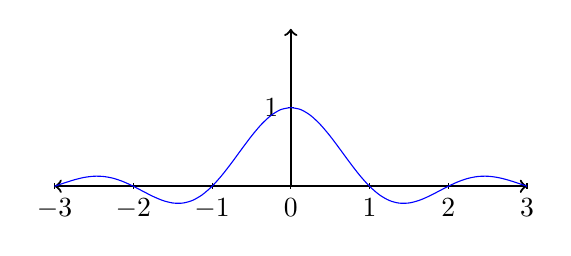
\begin{tikzpicture}
            \draw[thick,<->] (-3, 0) -- (3,0);
            \draw[thick,->] (0,0) -- (0,2);
            \foreach \x in {-3, -2, -1, 0, 1, 2, 3}
                \draw (\x ,1pt) -- (\x ,-1pt) node[anchor=north] {$\x$};
            \foreach \y in {1}
                \draw (1pt,\y cm) -- (-1pt,\y cm) node[anchor=east] {$\y$};
                \draw[scale=1,domain=-3:-0.001,smooth,variable=\x,blue] plot (\x,{sin((\x r * pi))/(\x * pi)});
                \draw[scale=1,domain=0.001:3,smooth,variable=\x,blue] plot (\x,{sin((\x r * pi))/(\x * pi)});
        \end{tikzpicture}
    \]
\end{definition}
Notice how the amplitude is attenuated further from zero. The sinc function is both differentiable and continuous.
Sinc interpolation will look something like this.
\[
    \begin{array}{ccc}
        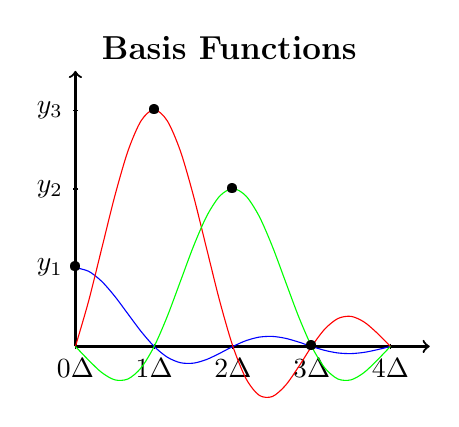
\begin{tikzpicture}
            \draw[thick,->] (0, 0) -- (4.5,0);
            \draw[thick,->] (0,0) -- (0,3.5);
            \foreach \x in {0,1, 2, 3, 4}
                \draw (\x cm,1pt) -- (\x cm,-1pt) node[anchor=north] {$\x \Delta$};
            \foreach \y in {1,2,3}
                \draw (1pt,\y cm) -- (-1pt,\y cm) node[anchor=east] {$y_{\y}$};
                \draw[scale=1,domain=0.001:4,smooth,variable=\x,blue] plot (\x,{sin((\x r * pi))/(\x * pi)});
                \draw[scale=1,domain=0.001:4,smooth,variable=\x,red] plot (\x,{3*sin(((\x - 1) r * pi))/((\x - 1) * pi)});
                \draw[scale=1,domain=0.001:4,smooth,variable=\x,green] plot (\x,{2*sin(((\x - 2) r * pi))/((\x - 2) * pi)});
            \foreach \Point in {(0,1), (2,2), (1,3), (3, 0)}{
                \node at \Point {\textbullet};
            }
            \node[above,font=\large\bfseries] at (current bounding box.north) {Basis Functions};
        \end{tikzpicture} &
        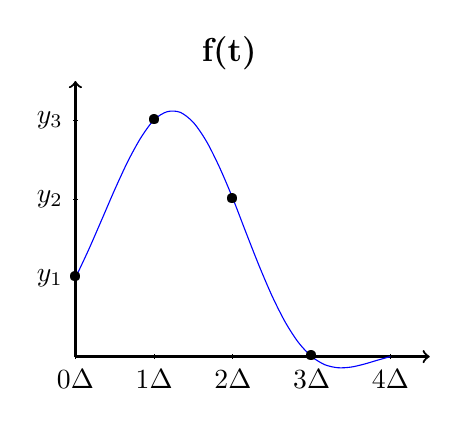
\begin{tikzpicture}
            \draw[thick,->] (0, 0) -- (4.5,0);
            \draw[thick,->] (0,0) -- (0,3.5);
            \foreach \x in {0,1, 2, 3, 4}
                \draw (\x cm,1pt) -- (\x cm,-1pt) node[anchor=north] {$\x \Delta$};
            \foreach \y in {1,2,3}
                \draw (1pt,\y cm) -- (-1pt,\y cm) node[anchor=east] {$y_{\y}$};
                \draw[scale=1,domain=0.001:4,smooth,variable=\x,blue] plot 
                (\x,{sin((\x r * pi))/(\x * pi) + 3*sin(((\x - 1) r * pi))/((\x - 1) * pi)+2*sin(((\x - 2) r * pi))/((\x - 2) * pi)});
            \foreach \Point in {(0,1), (2,2), (1,3), (3, 0)}{
                \node at \Point {\textbullet};
            }
            \node[above,font=\large\bfseries] at (current bounding box.north) {f(t)};
        \end{tikzpicture}
    \end{array}
\]
Another form of interpolation is polynomial interpolation where the datapoints are fit to a polynomial.
If we have $n$ datapoints, then our polynomial is $y(t) = \sum_{i=0}^{n}{a_i t^i}$
To fit this polynomial to our datapoints $(x_k, y_k)$, solve the system
\[
    \left[
        \begin{array}{ccccc}
            1 & x_0 & x_0^2 & ... & x_0^n\\
            1 & x_1 & x_1^2 & ... & x_1^n\\
            & & \vdots & &\\
            1 & x_n & x_n^2 & ... & x_n^n\\
        \end{array}
    \right]\left[
        \begin{array}{c}
            a_0\\
            a_1\\
            \vdots\\
            a_n\\
        \end{array}
    \right]=\left[
        \begin{array}{c}
            y_1\\
            y_2\\
            \vdots\\
            y_n\\
        \end{array}
    \right]
\]
The matrix on the left is called the Vandermonde matrix,
and it will always be invertible as long as there are no duplicate $(x_k, y_k)$.
While it might seem like polynomials are the best form of interpolation, they suffer heavily from
overfitting, so while they may perform well within samples, outside of the sample range, they degenerate very rapidly.
\end{document}
